\documentclass[12pt]{../notes}

% Command for Questions
%\question{}

% Command for Notes
% \note{}

% Code to create a minipage where you can type in class notes. 
%%\begin{minipage}[l][2cm][c]{\textwidth}
%\begin{comment}

%\end{comment}
%%\end{minipage}


% Begin Document
%==============================================================================
\begin{document}
% Include the Title of the Handout
\ntitle{3.3: Influential Observations and Outliers}

\question{Is it possible for a model outlier to not be reflected in a boxplot of $Y$? Explain why or why not.}

\begin{minipage}[l][2cm][c]{\textwidth}
%\begin{comment}
\note{Yes. A value of why can be exceptionally far away from the line \textit{given its X-values}, while still being in a reasonable range for Y overall.}
%\end{comment}
\end{minipage}

\nspace
Recall that $h_{i,l}$ represents the element in row $i$ and column $l$ of $H$\\
 - sometimes called ``leverage'' (influence of obs. $i$ on its
 fitted value)\\

Since $\hat{Y}=H Y$, then $\hat{Y}_i = \sum_{l=1}^{n} h_{i,l} Y_l$\\

\question{What would a ``larger'' diagonal element $h_{i,i}$ mean?}

\begin{minipage}[l][3cm][c]{\textwidth}
%\begin{comment}
\note{It means that the value of $Y_i$ is more influential in its own prediction ($\hat{Y}_i$). We care about this because if the influence of a particular point is large enough, then the model is likely fitting that particular point at the sacrifice of the rest of the data.}
%\end{comment}
\end{minipage}


\nspace
\question{What would cause an observation to have high leverage? (Hint: It has nothing to do with the values of Y.)}

\begin{minipage}[l][3cm][c]{\textwidth}
%\begin{comment}
\note{The technical answer is when the X-profile of the observation is far away from the point of averages for all X values (i.e. $\left(\bar{X}_1, \bar{X}_2, \ldots \bar{X}_{p-1}\right)$. In other words, it happens when an observation has an X-profile substantially different than all other observed X-profiles.}
%\end{comment}
\end{minipage}

\nspace 
\question{True or False (and explain): An observation with high leverage will have a large influence on the model fit, and an observation with low leverage will not have a large influence on the model fit.}

\begin{minipage}[l][3cm][c]{\textwidth}
%\begin{comment}
\note{False. Points with high leverage are good candidates for being influential points, but their status as an influential point needs to be verified by other measures of influence (DFFITS, Cooks D, etc.). Similarly, an observation that doesn't express high leverage may be influential for other reasons (such as an outlier Y value).}
%\end{comment}
\end{minipage}

For the remaining questions, please refer to Figure \ref{fig:influence} and assume the theoretical linear model $Y_i = \beta_0 + \beta_1X_i + \epsilon_i.$

\begin{figure}[H]
\centering
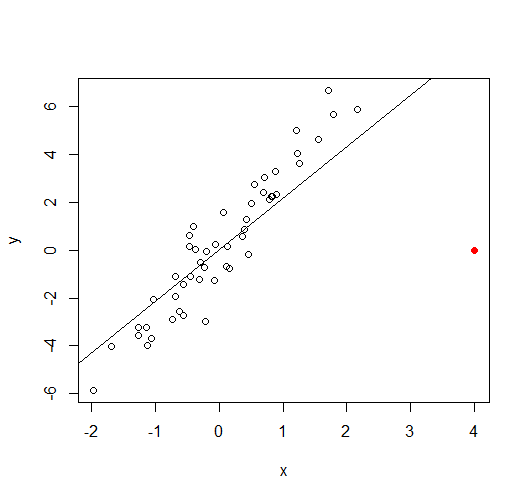
\includegraphics[width=0.5\textwidth]{../figures/module3/model_influence_example.png}
\caption{Sample scatterplot with estimated regression model.}
\label{fig:influence}
\end{figure}

\nspace
\question{Would the DFBETA associated with the filled in point be positive or negative? Explain.}

\begin{minipage}[l][2cm][c]{\textwidth}
%\begin{comment}
\note{Negative. This point is ``pulling'' the estimate of $\beta_1$ down, making it smaller than it would be if that observation was removed.}
%\end{comment}
\end{minipage}

\nspace
\question{Would the DFFITS associated with the filled in point be positive or negative? Explain.}

\begin{minipage}[l][2cm][c]{\textwidth}
%\begin{comment}
\note{Negative. The predicted value from the model at this point would be larger if this point was removed. Thus $\hat{Y}_i < \hat{Y}_{i(i)}$ which makes  $\hat{Y}_i - \hat{Y}_{i(i)} < 0$.}
%\end{comment}
\end{minipage}

\nspace
\question{Without any formal diagnostic checks, do you think that the filled in point is an outlier, influential point, both, or neither? Explain.}

\begin{minipage}[l][5cm][c]{\textwidth}
%\begin{comment}
\note{It is both an outlier and an influential point: 
\begin{itemize}
\item Outlier: The estimated value of Y is substantially farther away from the actual value of Y than the rest of the points. 
\item Influential Point: The observed value of X is very far away from the average value of X. Visually, we can see that this single point is compromising the trend that would be estimated for the rest of the data if that point was removed. 
\end{itemize}
}
%\end{comment}
\end{minipage}

% End the Document
%==============================================================================
\end{document}